% Generated by code/needham.py -- do not edit by hand.
\definecolor{qocA}{rgb}{0.00,0.45,0.70}
\definecolor{qocB}{rgb}{0.90,0.60,0.00}
\definecolor{qocC}{rgb}{0.00,0.62,0.45}
\definecolor{qocD}{rgb}{0.80,0.40,0.00}
\definecolor{qocE}{rgb}{0.80,0.60,0.70}
\definecolor{qocF}{rgb}{0.35,0.70,0.90}
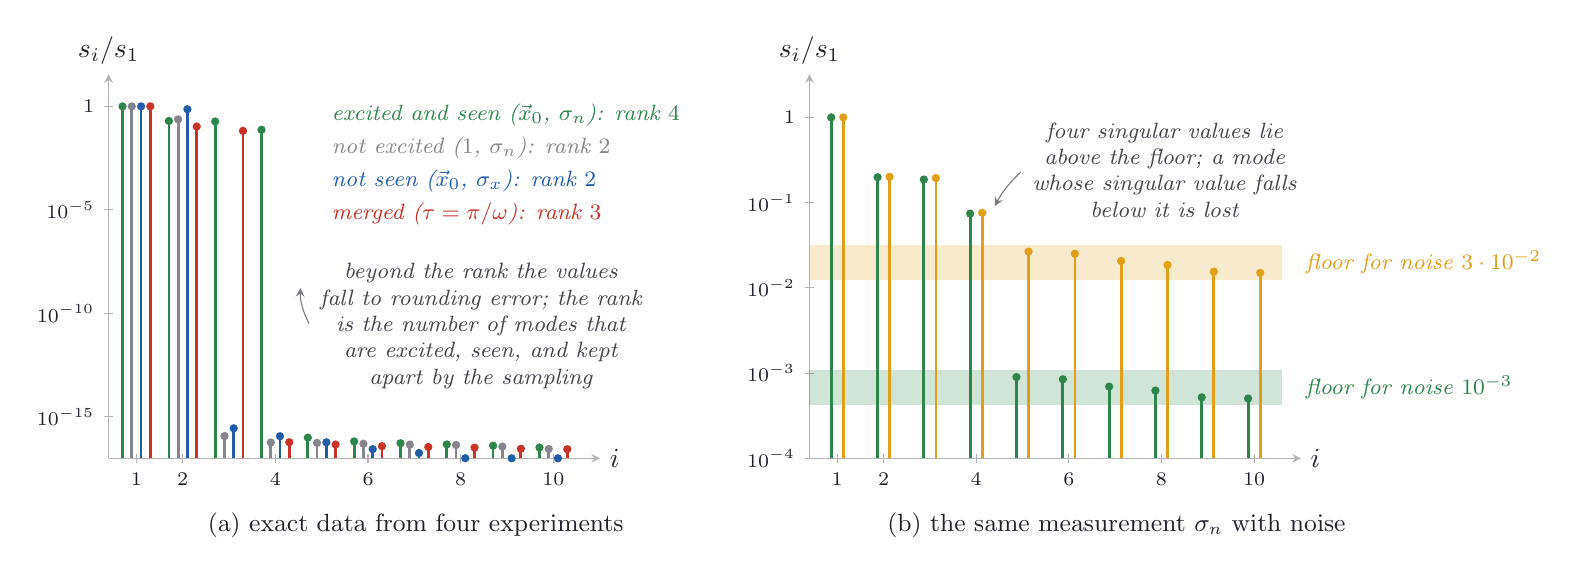
\begin{tikzpicture}[ink/.style={line width=0.9pt, ndInk}, faint/.style={line width=0.4pt, ndInk!35}, dashedink/.style={line width=0.5pt, ndInk!55, dash pattern=on 2.5pt off 2pt}, vec/.style={->, >=stealth, line width=1.2pt}, note/.style={font=\footnotesize\itshape, text=ndInk!85, align=center}, pointer/.style={->, >=stealth, line width=0.4pt, ndInk!60, shorten >=2pt, shorten <=1pt}, dot/.style={circle, fill=ndInk, inner sep=0pt, minimum size=3.4pt}, wash/.style={fill=ndSky, fill opacity=0.55}, every node/.style={text=ndInk}]
\definecolor{ndInk}{rgb}{0.13,0.13,0.18}
\definecolor{ndPaper}{rgb}{0.99,0.96,0.88}
\definecolor{ndSky}{rgb}{0.84,0.91,0.98}
\definecolor{ndRose}{rgb}{0.98,0.86,0.84}
\definecolor{ndBlue}{rgb}{0.13,0.36,0.66}
\definecolor{ndRed}{rgb}{0.78,0.20,0.16}
\definecolor{ndGold}{rgb}{0.88,0.62,0.10}
\definecolor{ndGreen}{rgb}{0.18,0.52,0.30}
\draw[faint, ->, >=stealth] (0.000,0.000) -- (6.240,0.000) node[right, text=ndInk] {$i$};
\draw[faint, ->, >=stealth] (0.000,0.000) -- (0.000,4.876) node[above, text=ndInk] {$s_i/s_1$};
\draw[faint] (0.353,0.060) -- (0.353,-0.060) node[below, font=\scriptsize, text=ndInk] {$1$};
\draw[faint] (0.941,0.060) -- (0.941,-0.060) node[below, font=\scriptsize, text=ndInk] {$2$};
\draw[faint] (2.118,0.060) -- (2.118,-0.060) node[below, font=\scriptsize, text=ndInk] {$4$};
\draw[faint] (3.294,0.060) -- (3.294,-0.060) node[below, font=\scriptsize, text=ndInk] {$6$};
\draw[faint] (4.471,0.060) -- (4.471,-0.060) node[below, font=\scriptsize, text=ndInk] {$8$};
\draw[faint] (5.647,0.060) -- (5.647,-0.060) node[below, font=\scriptsize, text=ndInk] {$10$};
\draw[faint] (0.060,4.469) -- (-0.060,4.469) node[left, font=\scriptsize, text=ndInk] {$1$};
\draw[faint] (0.060,3.154) -- (-0.060,3.154) node[left, font=\scriptsize, text=ndInk] {$10^{-5}$};
\draw[faint] (0.060,1.840) -- (-0.060,1.840) node[left, font=\scriptsize, text=ndInk] {$10^{-10}$};
\draw[faint] (0.060,0.526) -- (-0.060,0.526) node[left, font=\scriptsize, text=ndInk] {$10^{-15}$};
\draw[line width=1.0pt, ndGreen] (0.176,0.000) -- (0.176,4.469);
\fill[ndGreen] (0.176,4.469) circle (1.5pt);
\draw[line width=1.0pt, ndGreen] (0.765,0.000) -- (0.765,4.284);
\fill[ndGreen] (0.765,4.284) circle (1.5pt);
\draw[line width=1.0pt, ndGreen] (1.353,0.000) -- (1.353,4.277);
\fill[ndGreen] (1.353,4.277) circle (1.5pt);
\draw[line width=1.0pt, ndGreen] (1.941,0.000) -- (1.941,4.172);
\fill[ndGreen] (1.941,4.172) circle (1.5pt);
\draw[line width=1.0pt, ndGreen] (2.529,0.000) -- (2.529,0.262);
\fill[ndGreen] (2.529,0.262) circle (1.5pt);
\draw[line width=1.0pt, ndGreen] (3.118,0.000) -- (3.118,0.214);
\fill[ndGreen] (3.118,0.214) circle (1.5pt);
\draw[line width=1.0pt, ndGreen] (3.706,0.000) -- (3.706,0.191);
\fill[ndGreen] (3.706,0.191) circle (1.5pt);
\draw[line width=1.0pt, ndGreen] (4.294,0.000) -- (4.294,0.176);
\fill[ndGreen] (4.294,0.176) circle (1.5pt);
\draw[line width=1.0pt, ndGreen] (4.882,0.000) -- (4.882,0.160);
\fill[ndGreen] (4.882,0.160) circle (1.5pt);
\draw[line width=1.0pt, ndGreen] (5.471,0.000) -- (5.471,0.137);
\fill[ndGreen] (5.471,0.137) circle (1.5pt);
\draw[line width=1.0pt, ndInk!55] (0.294,0.000) -- (0.294,4.469);
\fill[ndInk!55] (0.294,4.469) circle (1.5pt);
\draw[line width=1.0pt, ndInk!55] (0.882,0.000) -- (0.882,4.304);
\fill[ndInk!55] (0.882,4.304) circle (1.5pt);
\draw[line width=1.0pt, ndInk!55] (1.471,0.000) -- (1.471,0.282);
\fill[ndInk!55] (1.471,0.282) circle (1.5pt);
\draw[line width=1.0pt, ndInk!55] (2.059,0.000) -- (2.059,0.201);
\fill[ndInk!55] (2.059,0.201) circle (1.5pt);
\draw[line width=1.0pt, ndInk!55] (2.647,0.000) -- (2.647,0.195);
\fill[ndInk!55] (2.647,0.195) circle (1.5pt);
\draw[line width=1.0pt, ndInk!55] (3.235,0.000) -- (3.235,0.185);
\fill[ndInk!55] (3.235,0.185) circle (1.5pt);
\draw[line width=1.0pt, ndInk!55] (3.824,0.000) -- (3.824,0.174);
\fill[ndInk!55] (3.824,0.174) circle (1.5pt);
\draw[line width=1.0pt, ndInk!55] (4.412,0.000) -- (4.412,0.169);
\fill[ndInk!55] (4.412,0.169) circle (1.5pt);
\draw[line width=1.0pt, ndInk!55] (5.000,0.000) -- (5.000,0.149);
\fill[ndInk!55] (5.000,0.149) circle (1.5pt);
\draw[line width=1.0pt, ndInk!55] (5.588,0.000) -- (5.588,0.118);
\fill[ndInk!55] (5.588,0.118) circle (1.5pt);
\draw[line width=1.0pt, ndBlue] (0.412,0.000) -- (0.412,4.469);
\fill[ndBlue] (0.412,4.469) circle (1.5pt);
\draw[line width=1.0pt, ndBlue] (1.000,0.000) -- (1.000,4.433);
\fill[ndBlue] (1.000,4.433) circle (1.5pt);
\draw[line width=1.0pt, ndBlue] (1.588,0.000) -- (1.588,0.381);
\fill[ndBlue] (1.588,0.381) circle (1.5pt);
\draw[line width=1.0pt, ndBlue] (2.176,0.000) -- (2.176,0.280);
\fill[ndBlue] (2.176,0.280) circle (1.5pt);
\draw[line width=1.0pt, ndBlue] (2.765,0.000) -- (2.765,0.203);
\fill[ndBlue] (2.765,0.203) circle (1.5pt);
\draw[line width=1.0pt, ndBlue] (3.353,0.000) -- (3.353,0.116);
\fill[ndBlue] (3.353,0.116) circle (1.5pt);
\draw[line width=1.0pt, ndBlue] (3.941,0.000) -- (3.941,0.067);
\fill[ndBlue] (3.941,0.067) circle (1.5pt);
\draw[line width=1.0pt, ndBlue] (4.529,0.000) -- (4.529,0.001);
\fill[ndBlue] (4.529,0.001) circle (1.5pt);
\draw[line width=1.0pt, ndBlue] (5.118,0.000) -- (5.118,0.000);
\fill[ndBlue] (5.118,0.000) circle (1.5pt);
\draw[line width=1.0pt, ndBlue] (5.706,0.000) -- (5.706,0.000);
\fill[ndBlue] (5.706,0.000) circle (1.5pt);
\draw[line width=1.0pt, ndRed] (0.529,0.000) -- (0.529,4.469);
\fill[ndRed] (0.529,4.469) circle (1.5pt);
\draw[line width=1.0pt, ndRed] (1.118,0.000) -- (1.118,4.213);
\fill[ndRed] (1.118,4.213) circle (1.5pt);
\draw[line width=1.0pt, ndRed] (1.706,0.000) -- (1.706,4.158);
\fill[ndRed] (1.706,4.158) circle (1.5pt);
\draw[line width=1.0pt, ndRed] (2.294,0.000) -- (2.294,0.204);
\fill[ndRed] (2.294,0.204) circle (1.5pt);
\draw[line width=1.0pt, ndRed] (2.882,0.000) -- (2.882,0.175);
\fill[ndRed] (2.882,0.175) circle (1.5pt);
\draw[line width=1.0pt, ndRed] (3.471,0.000) -- (3.471,0.154);
\fill[ndRed] (3.471,0.154) circle (1.5pt);
\draw[line width=1.0pt, ndRed] (4.059,0.000) -- (4.059,0.143);
\fill[ndRed] (4.059,0.143) circle (1.5pt);
\draw[line width=1.0pt, ndRed] (4.647,0.000) -- (4.647,0.135);
\fill[ndRed] (4.647,0.135) circle (1.5pt);
\draw[line width=1.0pt, ndRed] (5.235,0.000) -- (5.235,0.121);
\fill[ndRed] (5.235,0.121) circle (1.5pt);
\draw[line width=1.0pt, ndRed] (5.824,0.000) -- (5.824,0.115);
\fill[ndRed] (5.824,0.115) circle (1.5pt);
\node[note, anchor=west, text=ndGreen] at (2.71,4.36) {excited and seen ($\vec x_0$, $\sigma_n$): rank $4$};
\node[note, anchor=west, text=ndInk!55] at (2.71,3.94) {not excited ($\ket1$, $\sigma_n$): rank $2$};
\node[note, anchor=west, text=ndBlue] at (2.71,3.52) {not seen ($\vec x_0$, $\sigma_x$): rank $2$};
\node[note, anchor=west, text=ndRed] at (2.71,3.10) {merged ($\tau=\pi/\omega$): rank $3$};
\node[note, anchor=west] (c) at (2.56,1.68) {beyond the rank the values\\ fall to rounding error; the rank\\ is the number of modes that\\ are excited, seen, and kept\\ apart by the sampling};
\draw[pointer] (c.west) to[bend left=15] (2.441,2.234);
\node[font=\small] at (3.900,-0.850) {(a) exact data from four experiments};
\draw[faint, ->, >=stealth] (8.900,0.000) -- (15.140,0.000) node[right, text=ndInk] {$i$};
\draw[faint, ->, >=stealth] (8.900,0.000) -- (8.900,4.876) node[above, text=ndInk] {$s_i/s_1$};
\draw[faint] (9.253,0.060) -- (9.253,-0.060) node[below, font=\scriptsize, text=ndInk] {$1$};
\draw[faint] (9.841,0.060) -- (9.841,-0.060) node[below, font=\scriptsize, text=ndInk] {$2$};
\draw[faint] (11.018,0.060) -- (11.018,-0.060) node[below, font=\scriptsize, text=ndInk] {$4$};
\draw[faint] (12.194,0.060) -- (12.194,-0.060) node[below, font=\scriptsize, text=ndInk] {$6$};
\draw[faint] (13.371,0.060) -- (13.371,-0.060) node[below, font=\scriptsize, text=ndInk] {$8$};
\draw[faint] (14.547,0.060) -- (14.547,-0.060) node[below, font=\scriptsize, text=ndInk] {$10$};
\draw[faint] (8.960,4.329) -- (8.840,4.329) node[left, font=\scriptsize, text=ndInk] {$1$};
\draw[faint] (8.960,3.247) -- (8.840,3.247) node[left, font=\scriptsize, text=ndInk] {$10^{-1}$};
\draw[faint] (8.960,2.165) -- (8.840,2.165) node[left, font=\scriptsize, text=ndInk] {$10^{-2}$};
\draw[faint] (8.960,1.082) -- (8.840,1.082) node[left, font=\scriptsize, text=ndInk] {$10^{-3}$};
\draw[faint] (8.960,0.000) -- (8.840,0.000) node[left, font=\scriptsize, text=ndInk] {$10^{-4}$};
\fill[ndGreen, fill opacity=0.22] (8.900,0.673) rectangle (14.900,1.118);
\fill[ndGold, fill opacity=0.22] (8.900,2.269) rectangle (14.900,2.713);
\draw[line width=1.0pt, ndGreen] (9.176,0.000) -- (9.176,4.329);
\fill[ndGreen] (9.176,4.329) circle (1.5pt);
\draw[line width=1.0pt, ndGreen] (9.765,0.000) -- (9.765,3.569);
\fill[ndGreen] (9.765,3.569) circle (1.5pt);
\draw[line width=1.0pt, ndGreen] (10.353,0.000) -- (10.353,3.540);
\fill[ndGreen] (10.353,3.540) circle (1.5pt);
\draw[line width=1.0pt, ndGreen] (10.941,0.000) -- (10.941,3.107);
\fill[ndGreen] (10.941,3.107) circle (1.5pt);
\draw[line width=1.0pt, ndGreen] (11.529,0.000) -- (11.529,1.031);
\fill[ndGreen] (11.529,1.031) circle (1.5pt);
\draw[line width=1.0pt, ndGreen] (12.118,0.000) -- (12.118,1.003);
\fill[ndGreen] (12.118,1.003) circle (1.5pt);
\draw[line width=1.0pt, ndGreen] (12.706,0.000) -- (12.706,0.910);
\fill[ndGreen] (12.706,0.910) circle (1.5pt);
\draw[line width=1.0pt, ndGreen] (13.294,0.000) -- (13.294,0.860);
\fill[ndGreen] (13.294,0.860) circle (1.5pt);
\draw[line width=1.0pt, ndGreen] (13.882,0.000) -- (13.882,0.774);
\fill[ndGreen] (13.882,0.774) circle (1.5pt);
\draw[line width=1.0pt, ndGreen] (14.471,0.000) -- (14.471,0.760);
\fill[ndGreen] (14.471,0.760) circle (1.5pt);
\draw[line width=1.0pt, ndGold] (9.329,0.000) -- (9.329,4.329);
\fill[ndGold] (9.329,4.329) circle (1.5pt);
\draw[line width=1.0pt, ndGold] (9.918,0.000) -- (9.918,3.574);
\fill[ndGold] (9.918,3.574) circle (1.5pt);
\draw[line width=1.0pt, ndGold] (10.506,0.000) -- (10.506,3.559);
\fill[ndGold] (10.506,3.559) circle (1.5pt);
\draw[line width=1.0pt, ndGold] (11.094,0.000) -- (11.094,3.118);
\fill[ndGold] (11.094,3.118) circle (1.5pt);
\draw[line width=1.0pt, ndGold] (11.682,0.000) -- (11.682,2.626);
\fill[ndGold] (11.682,2.626) circle (1.5pt);
\draw[line width=1.0pt, ndGold] (12.271,0.000) -- (12.271,2.598);
\fill[ndGold] (12.271,2.598) circle (1.5pt);
\draw[line width=1.0pt, ndGold] (12.859,0.000) -- (12.859,2.506);
\fill[ndGold] (12.859,2.506) circle (1.5pt);
\draw[line width=1.0pt, ndGold] (13.447,0.000) -- (13.447,2.455);
\fill[ndGold] (13.447,2.455) circle (1.5pt);
\draw[line width=1.0pt, ndGold] (14.035,0.000) -- (14.035,2.371);
\fill[ndGold] (14.035,2.371) circle (1.5pt);
\draw[line width=1.0pt, ndGold] (14.624,0.000) -- (14.624,2.355);
\fill[ndGold] (14.624,2.355) circle (1.5pt);
\node[note, anchor=west, text=ndGreen] at (15.08,0.90) {floor for noise $10^{-3}$};
\node[note, anchor=west, text=ndGold] at (15.08,2.49) {floor for noise $3\cdot10^{-2}$};
\node[note, anchor=west] (f) at (11.61,3.66) {four singular values lie\\ above the floor; a mode\\ whose singular value falls\\ below it is lost};
\draw[pointer] (f.west) to[bend right=10] (11.224,3.140);
\node[font=\small] at (12.800,-0.850) {(b) the same measurement $\sigma_n$ with noise};
\end{tikzpicture}
